%!TEX program = xelatex
\documentclass{beamer}
\usepackage[UTF8]{ctex}
\usepackage{lmodern}
\usepackage{bm}
\mode<presentation> {
	
	% The Beamer class comes with a number of default slide themes
	% which change the colors and layouts of slides. Below this is a list
	% of all the themes, uncomment each in turn to see what they look like.
	
	%\usetheme{default}
	%\usetheme{AnnArbor}
	%\usetheme{Antibes}
	%\usetheme{Bergen}
	%\usetheme{Berkeley}
	%\usetheme{Berlin}
	%\usetheme{Boadilla}
	%\usetheme{CambridgeUS}
	\usetheme{Copenhagen}
	%\usetheme{Darmstadt}
	%\usetheme{Dresden}
	%\usetheme{Frankfurt}
	%\usetheme{Goettingen}
	%\usetheme{Hannover}
	%\usetheme{Ilmenau}
	%\usetheme{JuanLesPins}
	%\usetheme{Luebeck}
	%\usetheme{Madrid}
	%\usetheme{Malmoe}
	%\usetheme{Marburg}
	%\usetheme{Montpellier}
	%\usetheme{PaloAlto}
	%\usetheme{Pittsburgh}
	%\usetheme{Rochester}
	%\usetheme{Singapore}
	%\usetheme{Szeged}
	%\usetheme{Warsaw}
	
	% As well as themes, the Beamer class has a number of color themes
	% for any slide theme. Uncomment each of these in turn to see how it
	% changes the colors of your current slide theme.
	
	%\usecolortheme{albatross}
	%\usecolortheme{beaver}
	%\usecolortheme{beetle}
	%\usecolortheme{crane}
	%\usecolortheme{dolphin}
	%\usecolortheme{dove}
	%\usecolortheme{fly}
	%\usecolortheme{lily}
	%\usecolortheme{orchid}
	%\usecolortheme{rose}
	%\usecolortheme{seagull}
	%\usecolortheme{seahorse}
	%\usecolortheme{whale}
	%\usecolortheme{wolverine}
	
	%\setbeamertemplate{footline} % To remove the footer line in all slides uncomment this line
	%\setbeamertemplate{footline}[page number] % To replace the footer line in all slides with a simple slide count uncomment this line
	
	%\setbeamertemplate{navigation symbols}{} % To remove the navigation symbols from the bottom of all slides uncomment this line
}

\usepackage{graphicx} % Allows including images
\usepackage{booktabs} % Allows the use of \toprule, \midrule and \bottomrule in tables 
\usepackage[T1]{fontenc}
\usepackage{tabularray}
\UseTblrLibrary{booktabs}
\usepackage[utf8]{inputenc}
\setbeamertemplate{caption}[numbered]
\newcommand{\C}{\mathbb{C}}
\newcommand{\R}{\mathbb{R}}
\newcommand{\Q}{\mathbb{Q}}
\newcommand{\Z}{\mathbb{Z}}
\newcommand{\N}{\mathbb{N}}
\newcommand{\p}{\mathbb{P}}
\newcommand{\E}{\mathbb{E}}
\newcommand{\new}[1]{\textcolor{red}{#1}}
\usepackage{graphicx}
\usepackage{amssymb}
\usepackage{setspace}
\usepackage[toc,page]{appendix}
\usepackage{epstopdf}
\usepackage{latexsym}
\usepackage{amstext}
\usepackage{lmodern}
\usepackage{amsmath}
\usepackage{bbm}
\usepackage{amsfonts}
\usepackage{url}
\usepackage{bm}
\usepackage{mathrsfs}
\usepackage{mathtools}
\usepackage{float}
%\usepackage{hyperref} give reference hyperlink 
%\usepackage{setspace}
\usepackage{indentfirst}
\usepackage{multirow}
\usepackage{color}
\usepackage{mathtools}
% packages from template
\usepackage{amsmath,amsthm,amssymb,amsfonts}
\usepackage[width=.9\textwidth]{caption}
\usepackage{mathrsfs}
\usepackage{graphicx}
\newcommand{\indep}{\rotatebox[origin=c]{90}{$\models$}}
%\usepackage{textgreek}
\usepackage{bbold}
\usepackage{subcaption}
\usepackage{natbib}
\usepackage{verbatim}
\usepackage{soul}
\usepackage[utf8]{inputenc}
%\usepackage[algo2e,ruled,vlined]{algorithm2e} 
%\usepackage{fancyvrb}


\newtheorem{proposition}[theorem]{Proposition}

\newcommand{\M}{\boldsymbol{M}}
\newcommand{\rank}{\mathrm{rank}}
\newcommand{\rep}{\mathrm{rep}}
\newcommand{\PR}{\text{Pr}}
\newcommand{\pkg}[1]{{\fontseries{b}\selectfont #1}}
%\newcommand\norm[1]{\left\lVert#1\right\rVert}
\newcommand{\bs}[1]{\pmb{#1}}
\newcommand{\mb}[1]{\boldsymbol{#1}}
\DeclareMathOperator*{\argmin}{arg\,min}
\DeclarePairedDelimiter{\ceil}{\lceil}{\rceil}
\DeclarePairedDelimiterX{\norm}[1]{\lVert}{\rVert}{#1}
\allowdisplaybreaks
%=============================================================================
% prelude
%=============================================================================
\def\mathLarge#1{\mbox{\LARGE $#1$}}
\usepackage{soul}


\title[]{二维随机变量及其概率分布}
\author[概率统计]{张宏达}
\institute{Nanjing University}
\date{}
\begin{document}
	\begin{frame}
		\titlepage
	\end{frame}
	
	\begin{frame}
		\frametitle{主要内容}
		\begin{itemize}
			\item 二维随机变量的分布函数
			\item 二维离散型随机变量
			\item 二维连续型随机变量
			\item 条件分布
			\item 二维随机变量函数的分布
		\end{itemize}
	\end{frame}
	
	\begin{frame}
		定义 3.1 设 $(X, Y)$ 为二维随机变量, 对任意实数 $(x, y)$, 二元函数
		
		$$
		F(x, y)=P\{(X \leqslant x) \cap(Y \leqslant y)\}=P\{X \leqslant x, Y \leqslant y\}
		$$
		
		称为二维随机变量 $(X, Y)$ 的联合分布函数, 简称分布函数.
	\end{frame}
	
	\begin{frame}
		如果将 $(X, Y)$ 看成平面上随机点的坐标, 则分布画数 $F(x, y)$ 在 $(x, y)$ 处的函数值
		
		$$
		F(x, y)=P\{X \leqslant x, Y \leqslant y\}
		$$
		
		就是随机点 $(X, Y)$ 落入以 $(x, y)$ 为右上顶点的无穷短形区域的概率 (图 3-1)。
		\begin{figure}
			\centering
			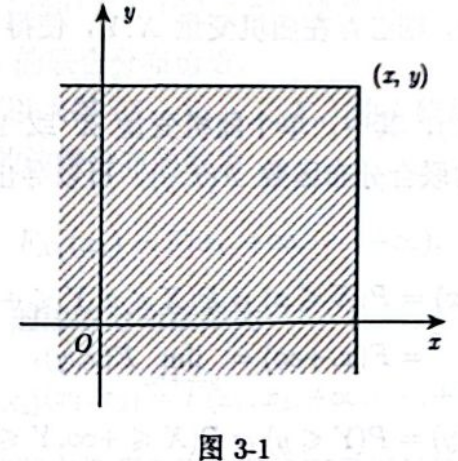
\includegraphics[scale = 0.3]{figures/figure3-1.jpg}
		\end{figure}
	\end{frame}
	
	\begin{frame}
		联合分布函数 $F(x, y)$ 具有以下基本性质:
		
		(1) $F(x, y)$ 分别是 $x$ 和 $y$ 的单调不减函数, 即对任意固定的 $y$, 当 $x_{2}>x_{1}$ 时, $F\left(x_{2}, y\right) \geqslant$ $F\left(x_{1}, y\right)$; 对任意固定的 $x$, 当 $y_{2}>y_{1}$ 时, 有 $F\left(x, y_{2}\right) \geqslant F\left(x, y_{1}\right)$ 。
		
		(2) $0 \leqslant F(x, y) \leqslant 1$, 且对任意固定的 $y, F(-\infty, y)=0$; 对任意固定的 $x, F(x,-\infty)=0$, 以及 $F(-\infty,-\infty)=0, F(+\infty,+\infty)=1$ 。 (3) $F(x, y)$ 关于 $x, y$ 右连续, 即
		
		$$
		F(x+0, y)=F(x, y), \quad F(x, y+0)=F(x, y) \text { 。 }
		$$
		
		(4) 对任意实数 $x_{2}>x_{1}, y_{2}>y_{1}$, 有
		
		$$
		F\left(x_{2}, y_{2}\right)-F\left(x_{1}, y_{2}\right)-F\left(x_{2}, y_{1}\right)+F\left(x_{1}, y_{1}\right) \geqslant 0 \text { 。 }
		$$
		
		性质 (1) 性质 (3) 与一维随机变量相似, 性质 (4) 反映了随机变量 $(X, Y)$ 在矩形区域取值 的概率非负 (图 3-2), 实际上
	\end{frame}
	
	\begin{frame}
	$$
	\begin{aligned}
		& P\left(x_{1}<X \leqslant x_{2}, y_{1}<Y \leqslant y_{2}\right) \\
		= & P\left(X \leqslant x_{2}, Y \leqslant y_{2}\right)-P\left(X \leqslant x_{1}, Y \leqslant y_{2}\right)-P\left(X \leqslant x_{2}, Y \leqslant y_{1}\right) \\ 
		& + \quad P\left(X \leqslant x_{1}, Y \leqslant y_{1}\right) \\
		= & F\left(x_{2}, y_{2}\right)-F\left(x_{1}, y_{2}\right)-F\left(x_{2}, y_{1}\right)+F\left(x_{1}, y_{1}\right) \geqslant 0 。
	\end{aligned}
	$$
	\begin{figure}
		\centering
		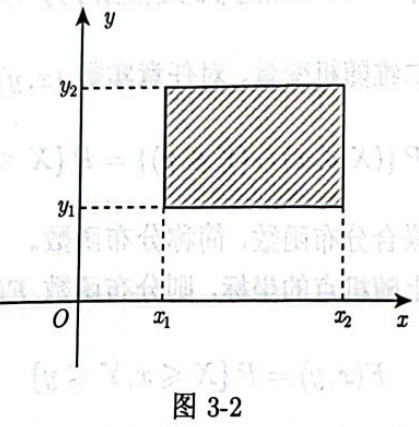
\includegraphics[scale=0.3]{figures/figure3-2.jpg}
	\end{figure}
	\end{frame}
	
	\begin{frame}
		对于二维随机变量 $(X, Y)$, 其中, 单个随机变量 $X$ 或 $Y$ 的分布称为\textbf{边缘分布}。若 已知二维随机变量 $(X, Y)$ 的联合分布函数 $F(x, y)$, 可以导出 $X$ 和 $Y$ 的边缘分布函数 $F_{X}(x), F_{Y}(y)$ :
		
		$$
		\begin{aligned}
			F_{X}(x) & =P(X \leqslant x)=P(X \leqslant x, Y \leqslant+\infty) \\
			& =F(x,+\infty)=\lim _{y \rightarrow+\infty} F(x, y), \\
			F_{Y}(y) & =P(Y \leqslant y)=P(X \leqslant+\infty, Y \leqslant y) \\
			& =F(+\infty, y)=\lim _{x \rightarrow+\infty} F(x, y) .
		\end{aligned}
		$$
	\end{frame}
	 
	\begin{frame}
		3.1 设二维随机变量 $(X, Y)$ 的联合分布函数为
		
		$$
		F(x, y)=A\left(B+\arctan \frac{x}{2}\right)\left(C+\arctan \frac{y}{3}\right), \quad-\infty<x, y<+\infty \text { 。 }
		$$
		(1) 求常数 $A, B, C$; 
		
		(2) 求 $X, Y$ 的边缘分布函数;
		
		(3) 求概率 $P(Y>3)$ 。
	\end{frame}
	
	\begin{frame}
		解 (1) 由分布函数的性质, 对任意 $x, y$ 有
		
		$$
		\begin{gathered}
			F(x,-\infty)=A\left(B+\arctan \frac{x}{2}\right)\left(C-\frac{\pi}{2}\right)=0, \\
			F(-\infty, y)=A\left(B-\frac{\pi}{2}\right)\left(C+\arctan \frac{y}{3}\right)=0, \\
			F(+\infty,+\infty)=A\left(B+\frac{\pi}{2}\right)\left(C+\frac{\pi}{2}\right)=1,
		\end{gathered}
		$$
		
		可以解得, $B=\frac{\pi}{2}, C=\frac{\pi}{2}, A=\frac{1}{\pi^{2}}$ 。
		
		(2) $X$ 的边缘分布函数为
		
		$$
		\begin{aligned}
			F_{X}(x) & =F(x,+\infty)=\lim _{y \rightarrow+\infty} \frac{1}{\pi^{2}}\left(\frac{\pi}{2}+\arctan \frac{x}{2}\right)\left(\frac{\pi}{2}+\arctan \frac{y}{3}\right) \\
			& =\frac{1}{\pi}\left(\frac{\pi}{2}+\arctan \frac{x}{2}\right), \quad-\infty<x<+\infty .
		\end{aligned}
		$$
		
		同理, $Y$ 的边缘分布函数为
		
		$$
		F_{Y}(y)=\frac{1}{\pi}\left(\frac{\pi}{2}+\arctan \frac{y}{3}\right), \quad-\infty<y<+\infty \text { 。 }
		$$
		
		
	\end{frame}
	\begin{frame}
		(3) $P(Y>3)=1-P(Y \leqslant 3)=1-F_{Y}(3)=1-\left(\frac{1}{2}+\frac{1}{\pi} \arctan 1\right)=\frac{1}{4}$ 。
	\end{frame}
	
	\begin{frame}
		二维分布函数的概念可以推广到 $n$ 维随机变量。
		
		定义 3.2 设 $\left(X_{1}, X_{2}, \cdots, X_{n}\right)$ 是 $n$ 维随机变量, 对任意实数 $x_{1}, x_{2}, \cdots, x_{n}$, 称 $n$ 维 函数
		
		$$
		F\left(x_{1}, x_{2}, \cdots, x_{n}\right)=P\left\{X_{1} \leqslant x_{1}, X_{2} \leqslant x_{2}, \cdots, X_{n} \leqslant x_{n}\right\}
		$$
		
		为随机变量 $\left(X_{1}, X_{2}, \cdots, X_{n}\right)$ 的联合分布函数。
		
		与二维情况类似, 我们可以求得 $\left(X_{1}, X_{2}, \cdots, X_{n}\right)$ 的 $k$ 维边缘分布函数 $(1 \leqslant k<n)$, 例 如, $\left(X_{1}, X_{2}, \cdots, X_{n}\right)$ 中 $X_{1}$ 的边缘分布函数为
		
		$$
		F_{X_{1}}\left(x_{1}\right)=F\left(x_{1},+\infty, \cdots,+\infty\right),
		$$
		
		$\left(X_{1}, X_{2}, \cdots, X_{n}\right)$ 中 $\left(X_{1}, X_{2}\right)$ 的边缘分布函数为
		
		$$
		F_{\left(X_{1}, X_{2}\right)}\left(x_{1}, x_{2}\right)=F\left(x_{1}, x_{2},+\infty, \cdots,+\infty\right) 。
		$$
	\end{frame}
	
	\begin{frame}
		定义 3.3 设随机变量 $X, Y$ 满足, 对任意 $x, y$, 随机事件 $X \leqslant x$ 与 $Y \leqslant y$ 独立, 即
		
		$$
		P(X \leqslant x, Y \leqslant y)=P(X \leqslant x) P(Y \leqslant y),
		$$
		
		即
		
		$$
		F(x, y)=F_{X}(x) F_{Y}(y)
		$$
		则称随机变量 $X, Y$ 相互独立。
		
		我们不加证明地给出随机变量独立性的一个重要性质: 若随机变量 $X, Y$ 相互独立, $f(x)$, $g(y)$ 为 $X, Y$ 的连续或分段连续函数, 则随机变量的函数 $f(X)$ 与 $g(Y)$ 相互独立。(随机变 量的函数的概念见本章第四节)
		
		例如, $X, Y$ 相互独立, 则 $X^{2}$ 与 $Y^{3}$ 相互独立, $\sin X$ 与 $\cos Y$ 相互独立。
		
		对于 $n$ 维随机变量 $\left(X_{1}, X_{2}, \cdots, X_{n}\right)$, 若对任意实数 $x_{1}, x_{2}, \cdots, x_{n}$, 有
		
		
	\end{frame}
	
	\begin{frame}
		\begin{align}
			& P\left(X_{1} \leqslant x_{1}, X_{2} \leqslant x_{2}, \cdots, X_{n} \leqslant x_{n}\right) \\
			&=P\left(X_{1} \leqslant x_{1}\right) P\left(X_{2} \leqslant x_{2}\right) \cdots P\left(X_{n} \leqslant x_{n}\right),
		\end{align}
		
		
		
		即
		
		$$
		F\left(x_{1}, x_{2}, \cdots, x_{n}\right)=F_{X_{1}}\left(x_{1}\right) F_{X_{2}}\left(x_{2}\right) \cdots F_{X_{n}}\left(x_{n}\right),
		$$
		
		则称 $X_{1}, X_{2}, \cdots, X_{n}$ 相互独立。
	\end{frame}
	
	\begin{frame}
		\frametitle{二维离散随机变量}
		定义 3.4 若二维随机变量 $(X, Y)$ 的可能取值是有限多个或可列无限多个, 则称 $(X, Y)$ 为离散型随机变量。
		
		定义 3.5 (离散型随机变量联合分布律) 设二维离散型随机变量 $(X, Y)$ 的所有可能取 值为 $\left(x_{i}, y_{j}\right), i, j=1,2, \cdots$, 则称
		
		$$
		P\left(X=x_{i}, Y=y_{j}\right)=p_{i j}, \quad i, j=1,2, \cdots
		$$
		为离散型随机变量 $(X, Y)$ 的联合分布律。
	\end{frame}
	
	\begin{frame}
		离散型随机变量的联合分布律具有如下性质:
		
		(1) $p_{i j} \geqslant 0, i, j=1,2, \cdots$;
		
		(2) $\sum_{i=1}^{\infty} \sum_{j=1}^{\infty} p_{i j}=1$ 。
		
	\end{frame}
	
	\begin{frame}
		在二维联合分布中, 可推导单个随机变量 $X$ 或 $Y$ 的分布律, 称为边缘分布律。
		
		$$
		\begin{aligned}
			P\left(X=x_{i}\right) & =P\left(X=x_{i}, Y<+\infty\right)=P\left(X=x_{i}, \bigcup_{j=1}^{\infty}\left(Y=y_{j}\right)\right) \\
			& =\sum_{j=1}^{\infty} P\left(X=x_{i}, Y=y_{j}\right)=\sum_{j=1}^{\infty} p_{i j} \stackrel{\text { 记为 }}{=} p_{i \bullet 。}
		\end{aligned}
		$$
		
		同理
		
		$$
		P\left(Y=y_{j}\right)=\sum_{i=1}^{\infty} P\left(X=x_{i}, Y=y_{j}\right)=\sum_{i=1}^{\infty} p_{i j} \stackrel{\text { 记为 }}{=} p_{\bullet j} \text { 。 }
		$$
	\end{frame}
	
	\begin{frame}
		二维离散型随机变量 $(X, Y)$ 的联合分布函数为
		
		$$
		F(x, y)=\sum_{x_{i} \leqslant x} \sum_{y_{j} \leqslant y} p_{i j}
		$$
		
		其中, 和式是对一切满足 $x_{i} \leqslant x, y_{j} \leqslant y$ 的 $i, j$ 求和。
		
		边缘分布函数为
		
		$$
		F_{X}(x)=\sum_{x_{i} \leqslant x}^{\infty} p_{i \bullet}=\sum_{x_{i} \leqslant x} \sum_{j=1}^{\infty} p_{i j}, \quad F_{Y}(y)=\sum_{y_{j} \leqslant y}^{\infty} p_{\bullet j}=\sum_{y_{j} \leqslant y} \sum_{i=1}^{\infty} p_{i j} \bullet
		$$
		
		二维离散型随机变量 $(X, Y)$ 在区域 $D$ 取值的概率可以表示为
		
		$$
		P((X, Y) \in D)=\sum_{\left(x_{i}, y_{j}\right) \in D} p_{i j} \text { 。 }
		$$
		
		二维离散型随机变量 $(X, Y)$ 的独立性等价于: 对任意 $i, j=1,2, \cdots$, 随机事件 $\left\{X=x_{i}\right\}$ 与 $\left\{Y=y_{j}\right\}$ 独立, 即
		
		$$
		P\left(X=x_{i}, Y=y_{j}\right)=P\left(X=x_{i}\right) P\left(Y=y_{j}\right), \quad i, j=1,2, \cdots,
		$$
		
		
	\end{frame}
	
	\begin{frame}
		即
		
		$$
		p_{i j}=p_{i \bullet} p_{\bullet j}, \quad i, j=1,2, \cdots 。
		$$
		
		例 3.2 将一枚硬币抛 3 次, 设 $X$ 是 3 次中正面出现的次数, $Y$ 表示出现正面次数与 反面次数之差的绝对值, 试求 $(X, Y)$ 的联合分布律及边缘分布律。
	\end{frame}
	
	\begin{frame}
		解 $X$ 的可能取值为 $0,1,2,3, Y=|X-(3-X)|=|2 X-3|, Y$ 的可能取值为 1,3 , 但 $(X, Y)$ 的可能取值只有 $(0,3),(1,1),(2,1),(3,3)$, 其他 $(X, Y)$ 取值概率为 0 。
		
		$$
		\begin{gathered}
			P(X=0, Y=3)=P(X=0)=\frac{1}{2^{3}}=\frac{1}{8}, \\
			P(X=1, Y=1)=P(X=1)=C_{3} \frac{1}{2^{3}}=\frac{3}{8}, \\
			P(X=2, Y=1)=P(X=2)=C_{3}^{2} \frac{1}{2^{3}}=\frac{3}{8} \\
			P(X=3, Y=3)=P(X=3)=\frac{1}{2^{3}}=\frac{1}{8} 。
		\end{gathered}
		$$
	\end{frame}
	
	\begin{frame}
		例 3.3 设随机变量 $X, Y$ 同分布, $X, Y \sim\left(\begin{array}{ccc}-1 & 0 & 1 \\ 0.25 & 0.5 & 0.25\end{array}\right)$, 已知 $P(X Y=0)=1$ 。
		
		(1) 求 $(X, Y)$ 的联合分布律;
		
		(2) 求 $P(X=Y)$;
		
		(3) 问 $X, Y$ 是否独立?
	\end{frame}
	
	\begin{frame}
		 (1) 设 $(X, Y)$ 的联合分布律为 $\because P(X Y=0)=1, \therefore P(X Y \neq 0)=0$,
		
		因此, $p_{11}=P(X=-1, Y=-1)=0$, 同理, $p_{13}=p_{31}=p_{33}=0$ 。
		
		由边缘分布得, $p_{12}=0.25, p_{21}=0.25, p_{23}=0.25, p_{32}=0.25, p_{22}=0$ 。
		
		(2) $P(X=Y)=p_{11}+p_{22}+p_{33}=0$ 。
		
		(3) 因为 $p_{22}=0$, 而 $p_{2 \bullet}=p_{\bullet 2}=0.5, p_{22} \neq p_{2 \bullet} \times p_{\bullet 2}$, 所以 $X, Y$ 不独立。
	\end{frame}
	
	\begin{frame}
		三项分布
		
		若二维离散型随机变量 $(X, Y)$ 的分布律为
		
		$$
		\begin{gathered}
			P(X=i, Y=j)=\frac{n !}{i ! j !(n-i-j) !} p_{1}^{i} p_{2}^{j}\left(1-p_{1}-p_{2}\right)^{n-i-j} \\
			i, j=0,1, \cdots, n, \quad i+j \leqslant n
		\end{gathered}
		$$
		
		其中, $0<p_{1}, p_{2}<1, p_{1}+p_{2}<1$, 则称 $(X, Y)$ 服从参数为 $n, p_{1}, p_{2}$ 的三项分布, 记为 $T\left(n, p_{1}, p_{2}\right)$ 。三项分布是二项分布的推广, 是多项分布的一种。
		
		在 $n$ 重独立试验中, 若每次试验有三种结果, $A_{1}, A_{2}, A_{3}, P\left(A_{i}\right)=p_{i}, p_{1}+p_{2}+p_{3}=1$, 设 $A_{1}$ 发生 $X$ 次, $A_{2}$ 发生 $Y$ 次, 则 $(X, Y)$ 服从三项分布。 $P(X=i, Y=j)$ 表示 $A_{1}$ 发生 $i$ 次, $A_{2}$ 发生 $j$ 次, $A_{3}$ 发生 $n-i-j$ 次的概率。
	\end{frame}
	
	\begin{frame}
		例 3.4 证明三项分布的边缘分布是二项分布, 即若 $(X, Y) \sim T\left(n, p_{1}, p_{2}\right)$, 则 $X \sim$ $B\left(n, p_{1}\right), Y \sim B\left(n, p_{2}\right)$ 。
	\end{frame}
	
	\begin{frame}
		证明 以 $X$ 的边缘分布为例, 对 $k=1,2, \cdots, n$
		
		$$
		\begin{aligned}
			& P(X=k)=\sum_{j=0}^{n-k} P(X=k, Y=j) \\
			= & \sum_{j=0}^{n-k} \frac{n !}{k ! j !(n-k-j) !} p_{1}^{k} p_{2}^{j}\left(1-p_{1}-p_{2}\right)^{n-k-j} \\
			= & \frac{n !}{k !(n-k) !} p_{1}^{k} \sum_{j=0}^{n-k} \frac{(n-k) !}{j ![(n-k)-j] !} p_{2}^{j}\left(1-p_{1}-p_{2}\right)^{(n-k)-j} \\
			= & \frac{n !}{k !(n-k) !} p_{1}^{k}\left(1-p_{1}\right)^{n-k}=C_{n}^{k} p_{1}^{k}\left(1-p_{1}\right)^{n-k}
		\end{aligned}
		$$
		
		可见, $X$ 服从二项分布 $B\left(n, p_{1}\right)$ 。
	\end{frame}
		
	\begin{frame}
		例 3.5 设 100 只产品中, 含有一、二、三等品分别为 $50,30,20$ 只, 从中有放回地抽 取 15 只, 求恰有一、三、三等品 $8,4,3$ 只的概率。
	\end{frame}
	
	\begin{frame}
		解:所抽取的 15 只产品中含有一、二等品的数目 $X, Y$ 服从三项分布 $T(15,0.5,0.3)$, 所求概率为
		
		$$
		P(X=8, Y=4)=\frac{15 !}{8 ! 4 ! 3 !} 0.5^{8} 0.3^{4} 0.2^{3}=0.0570 。
		$$
	\end{frame}
	
	\begin{frame}
		二维超几何分布
		
		若二维离散型随机变量 $(X, Y)$ 的分布律为
		
		$$
		P\left(X=n_{1}, Y=n_{2}\right)=\frac{C_{N_{1}}^{n_{1}} C_{N_{2}}^{n_{2}} C_{N_{3}}^{n_{3}}}{C_{N}^{n}},
		$$
		
		其中, $N=N_{1}+N_{2}+N_{3}, n=n_{1}+n_{2}+n_{3}$, 则称 $(X, Y)$ 服从二维超几何分布。
		
		总共 $N$ 个元素分为 $A, B, C$ 三类, 每类分别有 $N_{1}, N_{2}, N_{3}$ 个, 从中不放回地取出 $n$ 个, 设取到 $A$ 类 $X$ 个, $B$ 类 $Y$ 个, 则 $(X, Y)$ 服从二维超几何分布。 $P\left(X=n_{1}, Y=n_{2}\right)$ 表 示取到 $A$ 类 $n_{1}$ 个, $B$ 类 $n_{2}$ 个, $C$ 类 $n_{3}$ 个的概率。
	\end{frame}
	
	\begin{frame}
		例 3.6 设 100 只产品中, 含有一、二、三等品分别为 $50,30,20$ 只, 从中不放回地抽取 15 只, 求恰有一、三、三等品 $8,4,3$ 只的概率。
	\end{frame}
	
	\begin{frame}
		解:所抽取的 15 只产品中含有一、二等品的数目 $X, Y$ 服从二维超几何分布, 所求概 率为
		
		$$
		P(X=8, Y=4)=\frac{C_{50}^{8} C_{30}^{4} C_{20}^{3}}{C_{100}^{15}}=0.0662 。
		$$
		
		由例 3.5 和例 3.6 可见, 同样的问题, 由于抽样方式的不同, 分别服从三项分布和二维 超几何分布。
	\end{frame}
	 
	\begin{frame}
		\frametitle{二维连续型随机变量}
		定义 3.6 对于二维随机变量 $(X, Y)$ 的分布函数 $F(x, y)$, 如果存在非负函数 $p(x, y)$, 使得对于任意的 $(x, y)$ 有
		
		$$
		F(x, y)=\int_{-\infty}^{x} \int_{-\infty}^{y} p(u, v) \mathrm{d} u \mathrm{~d} v,
		$$
		
		则称 $(X, Y)$ 是二维连续型随机变量, 称 $p(x, y)$ 为 $(X, Y)$ 的联合概率密度函数。简称概率 密度。
	\end{frame}
	
	\begin{frame}
		二维连续型随机变量的联合概率密度具有下列性质:
		
		(1) $p(x, y) \geqslant 0$;
		
		(2) $\int_{-\infty}^{+\infty} \int_{-\infty}^{+\infty} p(x, y) \mathrm{d} x \mathrm{~d} y=F(+\infty,+\infty)=1$;
		
		(3) 设 $D$ 是平面区域, 则随机点 $(X, Y)$ 落入 $D$ 内的概率为
		
		$$
		P((X, Y) \in D)=\iint_{D} p(x, y) \mathrm{d} x \mathrm{~d} y ;
		$$
		
		(4) 若 $p(x, y)$ 在点 $(x, y)$ 处连续, 则有
		
		$$
		\frac{\partial^{2} F(x, y)}{\partial x \partial y}=p(x, y) 。
		$$
		
		由偏导数和积分性质, 当 $\Delta x, \Delta y$ 充分小时,
		
		$$
		\begin{aligned}
			& P(x<X \leqslant x+\Delta x, y<Y \leqslant y+\Delta y) \\
			= & \int_{x}^{x+\Delta x} \int_{y}^{y+\Delta y} p(u, v) \mathrm{d} u \mathrm{~d} v \approx p(x, y) \Delta x \Delta y,
		\end{aligned}
		$$
		
		因此, $p(x, y)$ 的大小反映了 $(X, Y)$ 落在点 $(x, y)$ 附近的
		\new{相对可能性}。
	\end{frame}
	
	\begin{frame}
		二、边缘密度及独立性条件
		
		在研究二维随机变量 $(X, Y)$ 时, $X$ 和 $Y$ 作为一维随机变量, 其概率密度称为边缘密 度, 分别记为 $p_{X}(x), p_{Y}(y)$ 。以下讨论边缘密度与联合密度的关系, 设 $X$ 和 $Y$ 的边缘分布 函数分别为 $F_{X}(x), F_{Y}(y)$, 则
		\begin{align}
			&F_{X}(x)=F(x,+\infty)=\int_{-\infty}^{x} \int_{-\infty}^{+\infty} p(t, y) \mathrm{d} t \mathrm{~d} y \\
			&=\int_{-\infty}^{x}\left[\int_{-\infty}^{+\infty} p(t, y) \mathrm{d} y\right] \mathrm{d} t
		\end{align}
		因此, $X$ 的边缘密度函数	
		$$
		p_{X}(x)=F_{X}^{\prime}(x)=\int_{-\infty}^{+\infty} p(x, y) \mathrm{d} y
		$$
		同理, $Y$ 的边缘密度函数
		$$
		p_{Y}(y)=F_{Y}^{\prime}(y)=\int_{-\infty}^{+\infty} p(x, y) \mathrm{d} x 。
		$$
	\end{frame}
	
	\begin{frame}
		随机变量 $X, Y$ 的 独立性条件为, 联合密度函数可以表示为边缘密度函数的乘积:
		
		$$
		F(x, y)=F_{X}(x) F_{Y}(y), \quad \forall(x, y),
		$$
		
		即
		
		$$
		\begin{aligned}
			\int_{-\infty}^{x} \int_{-\infty}^{y} p(u, v) \mathrm{d} u \mathrm{~d} v & =\int_{-\infty}^{x} p_{X}(t) \mathrm{d} t \int_{-\infty}^{y} p_{Y}(t) \mathrm{d} t \\
			& =\int_{-\infty}^{x} \int_{-\infty}^{y} p_{X}(x) p_{Y}(y) \mathrm{d} x \mathrm{~d} y 。
		\end{aligned}
		$$
		
		上式对任意 $(x, y)$ 成立, 因此得到用密度函数表示的独立性条件
		
		$$
		p(x, y)=p_{X}(x) p_{Y}(y), \quad \forall(x, y) 。
		$$
	\end{frame}
	
	\begin{frame}
		以上结果可以推广到 $n$ 维随机变量 $\left(X_{1}, X_{2}, \cdots, X_{n}\right)$ 。 
		
		定义 3.7 设 $\left(X_{1}, X_{2}, \cdots, X_{n}\right)$ 为 $n$ 维随机变量, 若存在非负函数 $p\left(x_{1}, x_{2}, \cdots, x_{n}\right)$ 使 得对任意实数 $x_{1}, x_{2}, \cdots, x_{n}$, 有
		
		$$
		F\left(x_{1}, x_{2}, \cdots, x_{n}\right)=\int_{-\infty}^{x_{1}} \int_{-\infty}^{x_{2}} \cdots \int_{-\infty}^{x_{n}} p\left(u_{1}, u_{2}, \cdots, u_{n}\right) \mathrm{d} u_{1} \mathrm{~d} u_{2} \cdots \mathrm{d} u_{n},
		$$
		
		则称 $\left(X_{1}, X_{2}, \cdots, X_{n}\right)$ 为 $n$ 维连续型随机变量, $p\left(x_{1}, x_{2}, \cdots, x_{n}\right)$ 为 $\left(X_{1}, X_{2}, \cdots, X_{n}\right)$ 的联 合密度函数。 $n$ 维密度函数的性质与二维密度函数相似, 不再一一列出。
	\end{frame}
	
	\begin{frame}
		与二维情况类似, 我们可以求得 $\left(X_{1}, X_{2}, \cdots, X_{n}\right)$ 的 $k$ 维边缘密度函数 $(1 \leqslant k<n)$, 例 如, $\left(X_{1}, X_{2}, \cdots, X_{n}\right)$ 中 $X_{1}$ 的边缘密度函数为
		
		$$
		p_{X_{1}}\left(x_{1}\right)=\int_{-\infty}^{+\infty} \int_{-\infty}^{+\infty} \cdots \int_{-\infty}^{+\infty} p\left(x_{1}, u_{2}, u_{3}, \cdots, u_{n}\right) \mathrm{d} u_{2} \mathrm{~d} u_{3} \cdots \mathrm{d} u_{n},
		$$
		
		$\left(X_{1}, X_{2}, \cdots, X_{n}\right)$ 中 $\left(X_{1}, X_{2}\right)$ 的边缘密度函数为
		
		$$
		p_{\left(X_{1}, X_{2}\right)}\left(x_{1}, x_{2}\right)=\int_{-\infty}^{+\infty} \int_{-\infty}^{+\infty} \cdots \int_{-\infty}^{+\infty} p\left(x_{1}, x_{2}, u_{3},\cdots, u_{n}\right) \mathrm{d} u_{3} \cdots \mathrm{d} u_{n} 。
		$$
		
		$n$ 维随机变量的独立性条件可以表示为: 若对任意实数 $x_{1}, x_{2}, \cdots, x_{n}$, 有
		
		$$
		p\left(x_{1}, x_{2}, \cdots, x_{n}\right)=p_{X_{1}}\left(x_{1}\right) p_{X_{2}}\left(x_{2}\right) \cdots p_{X_{n}}\left(x_{n}\right)
		$$
		
		则 $\left(X_{1}, X_{2}, \cdots, X_{n}\right)$ 相互独立。
	\end{frame}
	
	\begin{frame}
		例 3.7 设二维随机变量 $(X, Y)$ 的密度函数为
		
		$$
		p(x, y)=\left\{\begin{array}{cc}
			C e^{-(3 x+4 y)}, & x>0, y>0 \\
			0, & \text { 其他 }
		\end{array}\right. \text { 。 }
		$$
		
		试求:
		
		(1) 常数 $C$;
		
		(2) 联合分布函数 $F(x, y)$;
		
		(3) $P(X+Y \geqslant 1)$;
		
		(4) 问 $X, Y$ 是否独立?
	\end{frame}
	
	\begin{frame}
		解 (1) 由密度函数性质
		
		$$
		\begin{aligned}
			\int_{-\infty}^{+\infty} \int_{-\infty}^{+\infty} p(x, y) \mathrm{d} x \mathrm{~d} y & =C \int_{0}^{+\infty} \int_{0}^{+\infty} e^{-(3 x+4 y)} \mathrm{d} x \mathrm{~d} y \\
			& =C \int_{0}^{+\infty} e^{-3 x} \mathrm{~d} x \int_{0}^{+\infty} e^{-4 y} \mathrm{~d} y=\frac{C}{12}=1,
		\end{aligned}
		$$
		
		所以 $C=12$ 。
		
		(2) $x \leqslant 0$ 或 $y \leqslant 0$ 时,
		
		$$
		p(x, y)=0, \quad F(x, y)=\int_{-\infty}^{x} \int_{-\infty}^{y} p(u, v) \mathrm{d} u \mathrm{~d} v=0
		$$
		
		$x>0$ 且 $y>0$ 时,
		
		$$
		\begin{array}{r}
			F(x, y)=\int_{-\infty}^{x} \int_{-\infty}^{y} p(u, v) \mathrm{d} u \mathrm{~d} v=12 \int_{0}^{x} \mathrm{~d} u \int_{0}^{y} e^{-(3 u+4 v)} \mathrm{d} v \\
			=12 \int_{0}^{x} e^{-3 u} \mathrm{~d} u \int_{0}^{y} e^{-4 v} \mathrm{~d} v=\left(1-e^{-3 x}\right)\left(1-e^{-4 y}\right), \\
			\therefore F(x, y)=\left\{\begin{array}{cc}
				\left(1-e^{-3 x}\right)\left(1-e^{-4 y}\right), & x>0, y>0 \\
				0, & \text { 其他 }
			\end{array}\right.
		\end{array}
		$$
	\end{frame}
	
	\begin{frame}
		(3) $P(X+Y \geqslant 1)=1-P(X+Y<1)=1-12 \int_{0}^{1} \mathrm{~d} x \int_{0}^{1-x} e^{-(3 x+4 y)} \mathrm{d} y=4 e^{-3}-3 e^{-4}$ 。
		
		(4)
		
		$$
		\begin{gathered}
			F_{X}(x)=\lim _{y \rightarrow \infty} F(x, y)=\left\{\begin{array}{cc}
				\left(1-e^{-3 x}\right), & x>0 \\
				0, & x \leqslant 0
			\end{array},\right. \\
			F_{Y}(y)=\lim _{x \rightarrow \infty} F(x, y)=\left\{\begin{array}{cc}
				\left(1-e^{-4 y}\right), & y>0 \\
				0, & y \leqslant 0
			\end{array},\right.
		\end{gathered}
		$$
		
		显然, $F(x, y)=F_{X}(x) F_{Y}(y)$, 所以 $X, Y$ 相互独立。
		
		\new{也可由联合密度函数性质直接证得。}
	\end{frame}
	
	\begin{frame}
		例 3.8 设二维随机变量 $(X, Y)$ 的密度函数为
		
		$$
		p(x, y)=\left\{\begin{array}{cc}
			1 / 2, & (x, y) \in D \\
			0, & \text { 其他 }
		\end{array}\right.
		$$
		
		其中, 区域 $D$ 由 $\left\{y=\frac{1}{x}, y=0, x=1, x=e^{2}\right\}$ 围成 (图 3-3), 求 $X, Y$ 的边缘密度函数。
		
		\begin{figure}
			\centering
			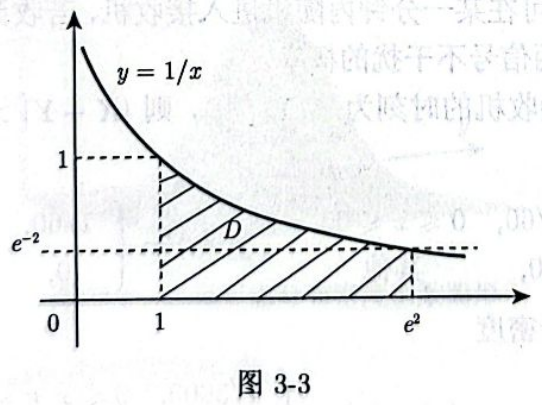
\includegraphics[scale = 0.3]{figures/figure3-3.jpg}
		\end{figure}
	\end{frame}
	
	\begin{frame}
		解 $p_{X}(x)=\int_{-\infty}^{+\infty} p(x, y) \mathrm{d} y$
		
		$$
		\begin{aligned}
			& =\left\{\begin{array}{c}
				\int_{0}^{1 / x} 1 / 2 \mathrm{~d} y, \quad 1 \leqslant x \leqslant e^{2} \\
				0, \quad \text { 其他 }
			\end{array}\right. \\
			& =\left\{\begin{array}{cc}
				\frac{1}{2 x}, & 1 \leqslant x \leqslant e^{2} \\
				0, & \text { 其他 }
			\end{array}\right.
		\end{aligned}
		$$
		
		$$
		p_{Y}(y)=\int_{-\infty}^{+\infty} p(x, y) \mathrm{d} x=\left\{\begin{array}{cc}
			\int_{1}^{e^{2}} \frac{1}{2} \mathrm{~d} x=\frac{1}{2}\left(e^{2}-1\right), & 0 \leqslant y \leqslant e^{-2} \\
			\int_{1}^{1 / y} \frac{1}{2} \mathrm{~d} x=\frac{1}{2}\left(\frac{1}{y}-1\right), & e^{-2} \leqslant y \leqslant 1 \\
			0, & \text { 其他 }
		\end{array} 。\right.
		$$
	\end{frame}
	
	\begin{frame}
	    二维均匀分布
		
		设 $D$ 为平面有界区域, 其面积为 $S_{D}$, 若二维连续型随机变量 $(X, Y)$ 的联合密度为
		$$
		p(x, y)=\left\{\begin{array}{cc}
			1 / S_{D}, & (x, y) \in D \\
			0, & \text { 其他 }
		\end{array},\right.
		$$
		
		则称 $(X, Y)$ 服从区域 $D$ 上的二维均匀分布。
		
		二维均匀分布的应用很广, 例如, 在圆 $C$ 内随机投点, 落点坐标 $(X, Y)$, 则 $(X, Y)$ 服 从圆 $C$ 上的二维均匀分布; 又如, 甲在 1 到 3 点之间, 乙在 2 到 4 点间随机到达某地, 到 达时刻分别为 $X, Y$, 则 $(X, Y)$ 服从区域 $[1,3] \times[2,4]$ 上的二维均匀分布。
		
		二维均匀分布的特点: 随机点落在 $D$ 内任一子区域 $D_{k}$ 的概率与 $D_{k}$ 的面积成正比, 与 $D_{k}$ 的形状和 $D_{k}$ 在 $D$ 内的位置无关, 这是因为
		
		$$
		P\left((X, Y) \in D_{k}\right)=\iint_{D_{k}} p(x, y) \mathrm{d} x \mathrm{~d} y=\iint_{D_{k}} 1 / S_{D} \mathrm{~d} x \mathrm{~d} y=S_{D_{k}} / S_{D} 。
		$$
		
		由此可见, 利用二维均匀分布所求概率结果为面积之比, 这正是平面上的几何概型求概 率的方法。
	\end{frame}
	
	\begin{frame}
		例 3.9 两独立信号可在某一分钟内随机进入接收机, 若收到两信号的时间间隔小于 5 秒, 则信号相互干扰, 求两信号不干扰的概率。
	\end{frame}
	
	\begin{frame}
		解:设两信号进入接收机的时刻为 $X, Y$ (秒), 则 $|X-Y|>5$ 时, 信号不干扰。由题 意, $X, Y \sim U[0,60]$,
		
		$$
		p_{X}(x)=\left\{\begin{array}{cc}
			1 / 60, & 0 \leqslant x \leqslant 60 \\
			0, & \text { 其他 }
		\end{array} \quad, \quad p_{Y}(y)=\left\{\begin{array}{cc}
			1 / 60, & 0 \leqslant y \leqslant 60 \\
			0, & \text { 其他 }
		\end{array},\right.\right.
		$$
		
		由 $X, Y$ 独立性, 联合密度
		
		$$
		\begin{aligned}
			& p(x, y)=p_{X}(x) p_{Y}(y)=\left\{\begin{array}{cc}
				1 / 3600, & 0 \leqslant x, y \leqslant 60 \\
				0, & \text { 其他 }
			\end{array},\right. \\
			& \begin{aligned}
				P(|X-Y|>5) & =\iint_{|x-y|>5} p(x, y) \mathrm{d} x \mathrm{~d} y \\
				& =\iint_{|x-y|>5} \frac{1}{3600} \mathrm{~d} x \mathrm{~d} y=\frac{1}{3600} S_{|x-y|>5} \\
				& =\frac{55^{2}}{3600}=0.8403,
			\end{aligned}
		\end{aligned}
		$$
		
		其中 $S_{|x-y|>5}=55^{2}$ (图 3-4)。
	\end{frame}
	
	\begin{frame}
		\begin{figure}
			\centering
			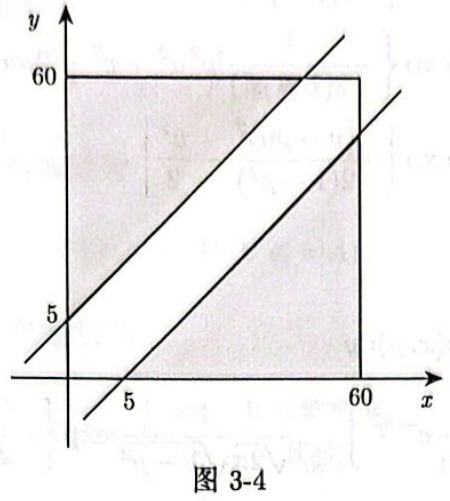
\includegraphics[scale = 0.3]{figures/figure3-4.jpg}
		\end{figure}
	\end{frame}
	
	\begin{frame}
		2. 二维正态分布
		
		若二维随机变量 $(X, Y)$ 的联合密度为
		
		$$
		\begin{aligned}
			p(x, y)= & \frac{1}{2 \pi \sigma_{1} \sigma_{2} \sqrt{1-\rho^{2}}} \exp \left\{-\frac{1}{2\left(1-\rho^{2}\right)}\left[\left(\frac{x-\mu_{1}}{\sigma_{1}}\right)^{2}\right.\right. \\
			& \left.\left.-2 \rho\left(\frac{x-\mu_{1}}{\sigma_{1}}\right)\left(\frac{y-\mu_{2}}{\sigma_{2}}\right)+\left(\frac{y-\mu_{2}}{\sigma_{2}}\right)^{2}\right]\right\},
		\end{aligned}
		$$
		
		其中, $\mu_{1}, \mu_{2}, \sigma_{1}>0, \sigma_{2}>0,|\rho|<1$ 均为常数, 则称 $(X, Y)$ 服从二维正态分布, 记为 $(X, Y) \sim N\left(\mu_{1}, \mu_{2}, \sigma_{1}^{2}, \sigma_{2}^{2}, \rho\right)$ (图 3-5)。
	\end{frame}
	
	\begin{frame}
		\begin{figure}
			\centering
			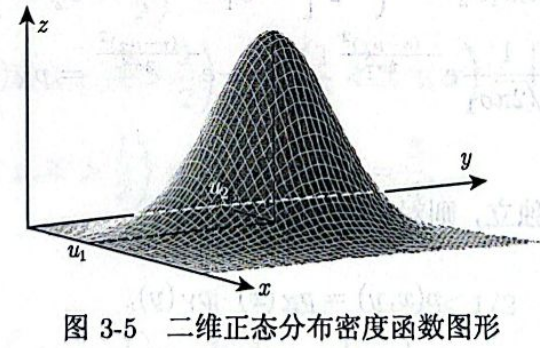
\includegraphics[scale = 0.3]{figures/figure3-5.jpg}
		\end{figure}
	\end{frame}
	
	\begin{frame}
		定理 3.1 设 $(X, Y)$ 服从二维正态分布 $N\left(\mu_{1}, \mu_{2}, \sigma_{1}^{2}, \sigma_{2}^{2}, \rho\right)$, 则 $X, Y$ 的边缘分布为 $X \sim N\left(\mu_{1}, \sigma_{1}^{2}\right), Y \sim N\left(\mu_{2}, \sigma_{2}^{2}\right) 。$
		
		\vspace*{1cm}
		证明 令 $u=\frac{x-\mu_{1}}{\sigma_{1}}, v=\frac{y-\mu_{2}}{\sigma_{2}}$, 则 $(X, Y)$ 的联合密度
		
		$$
		\begin{aligned}
			p(x, y)= & \frac{1}{2 \pi \sigma_{1} \sigma_{2} \sqrt{1-\rho^{2}}} \\
			& \cdot \exp \left\{-\frac{1}{2\left(1-\rho^{2}\right)}\left[\left(\frac{x-\mu_{1}}{\sigma_{1}}\right)^{2}-2 \rho\left(\frac{x-\mu_{1}}{\sigma_{1}}\right)\left(\frac{y-\mu_{2}}{\sigma_{2}}\right)\right.\right. \\
			&\quad + \left.\left.\left(\frac{y-\mu_{2}}{\sigma_{2}}\right)^{2}\right]\right\}
		\end{aligned}
		$$
	\end{frame}
	
	\begin{frame}
		$$
		\begin{aligned}
			& =\frac{1}{2 \pi \sigma_{1} \sigma_{2} \sqrt{1-\rho^{2}}} \exp \left[-\frac{1}{2\left(1-\rho^{2}\right)}\left(u^{2}-2 \rho u v+v^{2}\right)\right] \\
			& =\frac{1}{2 \pi \sigma_{1} \sigma_{2} \sqrt{1-\rho^{2}}} \exp \left\{-\frac{1}{2\left(1-\rho^{2}\right)}\left[\rho^{2} u^{2}+v^{2}-2 \rho u v
			\right.\right. \\
			& \quad\quad\quad +\left(1-\rho^{2}\right)
			\left.\left. u^{2}\right]\right\} \\
			& =\frac{1}{2 \pi \sigma_{1} \sigma_{2} \sqrt{1-\rho^{2}}} \exp \left[-\frac{(v-\rho u)^{2}}{2\left(1-\rho^{2}\right)}-\frac{u^{2}}{2}\right]
		\end{aligned}
		$$
		
		$X$ 的边缘密度为
		
		$$
		\begin{aligned}
			p_{X}(x) & =\int_{-\infty}^{+\infty} p(x, y) \mathrm{d} y \\
			& =\frac{1}{\sqrt{2 \pi} \sigma_{1}} e^{-\frac{u^{2}}{2}} \int_{-\infty}^{+\infty} \frac{1}{\sqrt{2 \pi} \sqrt{1-\rho^{2}}} \exp \left[-\frac{(v-\rho u)^{2}}{2\left(1-\rho^{2}\right)}\right] \mathrm{d} v
		\end{aligned}
		$$
	\end{frame}
	
	\begin{frame}
		因为积分中的被积函数是 $N\left(\rho u, 1-\rho^{2}\right)$ 的密度函数, 所以积分值为 1 , 从而,
		
		$$
		p_{X}(x)=\frac{1}{\sqrt{2 \pi} \sigma_{1}} e^{-\frac{u^{2}}{2}}=\frac{1}{\sqrt{2 \pi} \sigma_{1}} e^{-\frac{\left(x-\mu_{1}\right)^{2}}{2 \sigma_{1}^{2}}},
		$$
		
		即 $X \sim N\left(\mu_{1}, \sigma_{1}^{2}\right)$, 同理 $Y \sim N\left(\mu_{2}, \sigma_{2}^{2}\right)$ 。
	\end{frame}
	
	\begin{frame}
		定理 3.2 设 $(X, Y)$ 服从二维正态分布 $N\left(\mu_{1}, \mu_{2}, \sigma_{1}^{2}, \sigma_{2}^{2}, \rho\right)$, 则 $X, Y$ 相互独立的充要 条件为 $\rho=0$ 。
		
		证明:充分性: 设 $\rho=0$, 二维正态分布 $(X, Y)$ 的密度函数为
		
		$$
		\begin{aligned}
			p(x, y) & =\frac{1}{2 \pi \sigma_{1} \sigma_{2}} \exp \left\{-\frac{1}{2}\left[\frac{\left(x-\mu_{1}\right)^{2}}{\sigma_{1}^{2}}+\frac{\left(y-\mu_{2}\right)^{2}}{\sigma_{2}^{2}}\right]\right\} \\
			& =\frac{1}{\sqrt{2 \pi} \sigma_{1}} e^{-\frac{\left(x-\mu_{1}\right)^{2}}{2 \sigma_{1}^{2}}} \cdot \frac{1}{\sqrt{2 \pi} \sigma_{2}} e^{-\frac{\left(y-\mu_{2}\right)^{2}}{2 \sigma_{2}^{2}}}=p_{X}(x) p_{Y}(y),
		\end{aligned}
		$$
		
		所以, $X$ 与 $Y$ 相互独立。
		
		必要性: 设 $X, Y$ 相互独立, 则对任意实数 $x, y$ 有
		
		$$
		p(x, y)=p_{X}(x) \cdot p_{Y}(y)
		$$
		
		特别地, 令 $x=\mu_{1}, y=\mu_{2}$, 由 $p\left(\mu_{1}, \mu_{2}\right)=p_{X}\left(\mu_{1}\right) \cdot p_{Y}\left(\mu_{2}\right)$ 得到;
		
		$$
		\frac{1}{2 \pi \sigma_{1} \sigma_{2} \sqrt{1-\rho^{2}}}=\frac{1}{\sqrt{2 \pi} \sigma_{1}} \cdot \frac{1}{\sqrt{2 \pi} \sigma_{2}}
		$$
		
		从而得到 $\rho=0$ 。
	\end{frame}
	
	\begin{frame}
		\frametitle{条件分布}
		在随机事件的研究中, 讨论了条件概率问题, 而在随机变量的研究中, 可以类似讨论条 件分布问题。
		
		一、离散型随机变量的条件分布
		
		设 $(X, Y)$ 为二维离散型随机变量, 其概率分布律为
		
		$$
		P\left(X=x_{i}, Y=y_{j}\right)=p_{i j}, \quad i, j=1,2, \cdots 。
		$$
		
		当 $P\left(Y=y_{j}\right)=p_{\bullet j}>0$ 时, 可得
		
		$$
		P\left(X=x_{i} \mid Y=y_{j}\right)=\frac{P\left(X=x_{i}, Y=y_{j}\right)}{P\left(Y=y_{j}\right)}=\frac{p_{i j}}{p_{\bullet j}}, \quad i=1,2, \cdots,
		$$
		
		称为 $Y=y_{j}$ 条件下, 随机变量 $X$ 的条件分布律, 可记为
	\end{frame}
	
	\begin{frame}
		\begin{tabular}{c | c c c c c}
			$\left.X\right|_{Y=y_{j}}$ & $x_{1}$ & $x_{2}$ & $\cdots$ & $x_{i}$ & $\cdots$ \\
			\hline
			$P$ & $p_{1 j} / p_{\bullet j}$ & $p_{2 j} / p_{\bullet j}$ & $\cdots$ & $p_{i j} / p_{\bullet j}$ & $\cdots$ \\
		\end{tabular}
		
		同样, 当 $P\left(X=x_{i}\right)=p_{i \bullet}>0$ 时, 可得
		
		$$
		P\left(Y=y_{j} \mid X=x_{i}\right)=\frac{P\left(X=x_{i}, Y=y_{j}\right)}{P\left(X=x_{i}\right)}=\frac{p_{i j}}{p_{i \bullet}}, \quad j=1,2, \cdots,
		$$
		
		称为 $X=x_{i}$ 条件下, 随机变量 $Y$ 的条件分布律, 可记为
		\begin{tabular}{c|ccccc}
			$\left.Y\right|_{X=x_{i}}$ & $y_{1}$ & $y_{2}$ & $\cdots$ & $y_{j}$ & $\cdots$ \\
			\hline
			$P$ & $p_{i 1} / p_{i \bullet}$ & $p_{i 2} / p_{i \bullet}$ & $\cdots$ & $p_{i j} / p_{i \bullet}$ & $\cdots$ \\
		\end{tabular}
	\end{frame}
	
	\begin{frame}
		 $X, Y$ 相互独立时, $p_{i j}=p_{i \bullet} p_{\bullet j}$, 有
		
		$$
		P\left(X=x_{i} \mid Y=y_{j}\right)=\frac{p_{i j}}{p_{\bullet j}}=\frac{p_{i \bullet} p_{\bullet j}}{p_{\bullet j}}=p_{i \bullet}=P\left(X=x_{i}\right),
		$$
		
		同样
		
		$$
		P\left(Y=y_{j} \mid X=x_{i}\right)=p_{\bullet j}=P\left(Y=y_{j}\right),
		$$
		
		所以, 当 $X, Y$ 独立时, 条件分布成为无条件分布。
	\end{frame}
	
	\begin{frame}
		例 $3.11(X, Y)$ 的联合分布律如下, 求 $Y=1$ 条件下 $X$ 的条件分布律。
		\begin{figure}
			\centering
			\includegraphics[scale = 0.3]{figures/figure3-51.jpg}
		\end{figure}
	\end{frame}
	
	\begin{frame}
		解 $P(Y=1)=\frac{5}{8}, P\left(X=x_{i} \mid Y=y_{j}\right)=\frac{p_{i j}}{p_{\bullet j}}$, 因此
		
		$$
		\begin{gathered}
			P(X=1 \mid Y=1)=\frac{1 / 16}{5 / 8}=\frac{1}{10}, \quad P(X=2 \mid Y=1)=\frac{3 / 16}{5 / 8}=\frac{3}{10}, \\
			P(X=3 \mid Y=1)=\frac{1 / 8}{5 / 8}=\frac{1}{5}, \quad P(X=4 \mid Y=1)=\frac{1 / 4}{5 / 8}=\frac{2}{5},
		\end{gathered}
		$$
		
		所求条件分布律为
		\begin{tabular}{c|cccc}
			$\left.X\right|_{Y=1}$ & 1 & 2 & 3 & 4 \\
			\hline
			$P$ & $1 / 10$ & $3 / 10$ & $1 / 5$ & $2 / 5$ \\
		\end{tabular}
	\end{frame}
	
	\begin{frame}
	二、连续型随机变量的条件分布
	
	对于二维连续型随机变量 $(X, Y)$, 由于 $P(Y=y)=0$, 因此不能直接用
	
	$$
	P(X \leqslant x \mid Y=y)=\frac{P(X \leqslant x, Y=y)}{P(Y=y)}
	$$
	
	来定义 $Y=y$ 时 $X$ 的条件分布函数。
	
	定义 3.8 对给定的 $y$, 设 $\varepsilon>0$, 若对任意 $x$, 极限
	
	$$
	\lim _{\varepsilon \rightarrow 0} P(X \leqslant x \mid y \leqslant Y<y+\varepsilon)=\lim _{\varepsilon \rightarrow 0} \frac{P(X \leqslant x, y \leqslant Y<y+\varepsilon)}{P(y \leqslant Y<y+\varepsilon)}
	$$
	
	存在, 则称为 $Y=y$ 条件下, $X$ 的条件分布函数, 记为 $F_{X \mid Y=y}(x)$ 。
	\end{frame}
	
	\begin{frame}
		 $Y=y$ 条件下, $X$ 的\textbf{条件密度函数}, 记为 $p_{X \mid Y=y}(x)$,
		
		$$
		p_{X \mid Y=y}(x)=\frac{p(x, y)}{p_{Y}(y)} 。
		$$
		
		类似可得, 在 $X=x$ 条件下, $Y$ 的条件分布函数、条件密度函数分别为
		
		$$
		\begin{gathered}
			F_{Y \mid X=x}(y)=\int_{-\infty}^{y} \frac{p(x, v)}{p_{X}(x)} \mathrm{d} v, \\
			p_{Y \mid X=x}(y)=\frac{p(x, y)}{p_{X}(x)} 。
		\end{gathered}
		$$
		
		当 $X, Y$ 相互独立时, $p(x, y)=p_{X}(x) p_{Y}(y)$, 从而
		
		$$
		p_{X \mid Y=y}(x)=\frac{p(x, y)}{p_{Y}(y)}=p_{X}(x), \quad p_{Y \mid X=x}(y)=\frac{p(x, y)}{p_{X}(x)}=p_{Y}(y),
		$$
		
		条件密度成为无条件密度。
	\end{frame}
	
	\begin{frame}
		例 3.12 设随机变量 $(X, Y)$ 的密度函数为
		
		$$
		p(x, y)=\left\{\begin{array}{ll}
			e^{-y}, & 0<x<y \\
			0, & \text { 其他 }
		\end{array},\right.
		$$
		求 $Y=y$ 条件下, $X$ 的条件密度函数与条件分布函数。
	\end{frame}
	
	\begin{frame}
		解 $p_{Y}(y)=\int_{-\infty}^{+\infty} p(x, y) \mathrm{d} x=\int_{0}^{y} e^{-y} \mathrm{~d} x=y e^{-y}, \quad y>0$,
		
		当 $y>0$ 时, 由式 $(3.21), p_{X \mid Y=y}(x)=\frac{p(x, y)}{p_{Y}(y)}=\left\{\begin{array}{ll}1 / y, & 0<x<y \\ 0, & \text { 其他 }\end{array}\right.$ ,
		
		由式 (3.20), $F_{X \mid Y=y}(x)=\int_{-\infty}^{x} p_{X \mid Y=y}(u) \mathrm{d} u=\left\{\begin{array}{ll}0, & x \leqslant 0 \\ \int_{0}^{x} \frac{1}{y} \mathrm{~d} u=\frac{x}{y}, & 0<x<y \\ 1, & x \geqslant y\end{array}\right.$ 。
	\end{frame}
	
	\begin{frame}
		\frametitle{二维随机变量函数的分布}
		一、离散型随机变量函数的分布
		
		设二维离散型随机变量 $(X, Y)$ 的分布律为
		
		$$
		P\left(X=x_{i}, Y=y_{j}\right)=p_{i j}, \quad i, j=1,2, \cdots 。
		$$
		
		若 $(X, Y)$ 的函数 $Z=g(X, Y)$, 设 $Z$ 的可能取值为 $z_{k}, k=1,2, \cdots$, 则 $Z$ 的概率分布为
		
		$$
		\begin{aligned}
			P\left(Z=z_{k}\right) & =P\left(g(X, Y)=z_{k}\right) \\
			& =\sum_{g\left(x_{i}, y_{j}\right)=z_{k}} P\left(X=x_{i}, Y=y_{j}\right)=\sum_{g\left(x_{i}, y_{j}\right)=z_{k}} p_{i j} 。
		\end{aligned}
		$$
	\end{frame}
	
	\begin{frame}
		例 3.14 设随机变量 $(X, Y)$ 的联合分布律为
		
		$$
		P(X=i, Y=j)=\frac{1}{34}|3 i-4 j|, \quad i, j=1,2,3 。
		$$
		
		求 $Z=X+Y$ 的分布律。
	\end{frame}

	\begin{frame}
		解:分布律列表并将 $Z=X+Y$ 的值写在 $(X, Y)$ 相应处, 记为 $(Z)$
		
		\begin{tabular}{c|ccc}
			
			& X = 1 & X = 2 & X = 3 \\
			\hline
			Y = 1 & $1 / 34(2)$ & $5 / 34(3)$ & $9 / 34(4)$   \\
			Y = 2 & $2 / 34(3)$ & $2 / 34(4)$ & $6 / 34(5)$    \\
			Y = 3 & $5 / 34(4)$ & $1 / 34(5)$ & $3 / 34(6)$    \\
		\end{tabular}
		
		相同的 $(Z)$ 对应的概率值相加,
		
		\begin{tabular}{c|ccccc}
			$Z$ & 2 & 3 & 4 & 5 & 6 \\
			\hline
			$P$ & $1 / 34$ & $2 / 34+5 / 34$ & $5 / 34+2 / 34+9 / 34$ & $1 / 34+6 / 34$ & $3 / 34$ \\
		\end{tabular}
		
		得到
		
		\begin{tabular}{c|ccccc}
			$Z$ & 2 & 3 & 4 & 5 & 6 \\
			\hline
			$P$ & $1 / 34$ & $7 / 34$ & $16 / 34$ & $7 / 34$ & $3 / 34$ \\
		\end{tabular}
	\end{frame}
	
	\begin{frame}
		例 3.15 设 $X$ 和 $Y$ 独立, 均服从几何分布 $P(X=k)=P(Y=k)=p q^{k-1}(k=$ $1,2, \cdots)$, 试求 $Z=\max (X, Y)$ 的概率分布律。
	\end{frame}
	
	\begin{frame}
		\new{解:}
		$Z \leq n \Leftrightarrow X \leq n \cap Y \leq n$。
		$P(Z \leq n ) = P(X \leq n \cap Y \leq n) = P(X \leq n) P(Y \leq n) = (1 - q ^ n) ^2$
		\begin{align}
			P( Z = n ) & = P(Z \leq n) - P(Z \leq n - 1) \\
			& = (1 - q ^ n) ^2 - (1 - q ^ {n - 1}) ^2 \\
			& = pq ^ {n - 1}(2 - q ^ n - q ^ {n - 1})
		\end{align}
	\end{frame}
	
	\begin{frame}
		例 3.16 设 $X$ 和 $Y$ 独立, 分别服从参数为 $\lambda_{1}$ 和 $\lambda_{2}$ 泊松分布, 试求 $Z=X+Y$ 的 概率分布律。
	\end{frame}
	
	\begin{frame}
		解 $X$ 与 $Y$ 的可能取值都是 $0,1,2, \cdots$, 所以 $Z=X+Y$ 的所有可能取值也是 $0,1,2, \cdots$, 对任意 $n=0,1,2, \cdots$,
		
		$$
		\begin{aligned}
			P(Z=n) & =P(X+Y=n)=P\left(\bigcup_{k=0}^{n}(X=k, Y=n-k)\right) \\
			& =\sum_{k=0}^{n} P(X=k) P(Y=n-k)=\sum_{k=0}^{n} \frac{\lambda_{1}^{k}}{k !} e^{-\lambda_{1}} \frac{\lambda_{2}^{n-k}}{(n-k) !} e^{-\lambda_{2}} \\
			& =\frac{e^{-\left(\lambda_{1}+\lambda_{2}\right)}}{n !} \sum_{k=0}^{n} \frac{n !}{k !(n-k) !} \lambda_{1}^{k} \lambda_{2}^{n-k} \\
			& =\frac{e^{-\left(\lambda_{1}+\lambda_{2}\right)}}{n !}\left(\lambda_{1}+\lambda_{2}\right)^{n} 。
		\end{aligned}
		$$
		
		所以, $Z=X+Y$ 服从参数为 $\lambda_{1}+\lambda_{2}$ 的泊松分布, 这称为泊松分布的可加性。
	\end{frame}
	
	\begin{frame}
		泊松分布的 可加性可以推广到 $n$ 个独立泊松分布随机变量的情况, 即若随机变量 $X_{1}, X_{2}, \cdots, X_{n}$ 相互 独立, $X_{k} \sim P\left(\lambda_{k}\right), k=1,2, \cdots, n$, 则
		
		$$
		X_{1}+X_{2}+\cdots+X_{n} \sim P\left(\lambda_{1}+\lambda_{2}+\cdots+\lambda_{n}\right) \text { 。 }
		$$
		
		另外, 我们不加证明地给出结论, 二项分布也具有分布可加性: 若 $X \sim B\left(k_{1}, p\right), Y \sim$ $B\left(k_{2}, p\right)$ 且 $X, Y$ 独立, 则 $Z=X+Y \sim B\left(k_{1}+k_{2}, p\right)$ 。同样, 二项分布的可加性也能推广到 $n$ 个 独立随机变量的情形, 即若随机变量 $X_{1}, X_{2}, \cdots, X_{n}$ 相互独立, $X_{i} \sim B\left(k_{i}, p\right), i=1,2, \cdots, n$, 则
		
		$$
		X_{1}+X_{2}+\cdots+X_{n} \sim B\left(k_{1}+k_{2}+\cdots+k_{n}, p\right)
		$$
	\end{frame}
	
	\begin{frame}
		二、连续型随机变量函数的分布
		
		对于二维连续型随机变量 $(X, Y)$, 其函数 $Z=g(X, Y)$ 可能是离散型, 也可能是连续 型。对于离散型的情况, 可以按照 $Z$ 的每个取值, 根据相应 $(X, Y)$ 的取值范围, 分别求其 概率, 得到 $Z$ 的分布律, 通过例子说明。
		
		\vspace*{1cm}
		例 3.17 设 $(X, Y)$ 服从区域 $D=\{-1 \leqslant x \leqslant 2,-3 \leqslant y \leqslant 1\}$ 上的均匀分布, $Z=\{k$, 当 $(X, Y) \in$ 第 $k$ 象限, $k=1,2,3,4\}$, 求 $Z$ 的分布律。
	\end{frame}
	
	\begin{frame}
		解
			\begin{figure}
				\centering
				\includegraphics[scale = 0.15]{figures/figure3-52.jpg}
			\end{figure}
		$$
		\begin{aligned}
			& P(Z=1)=P((X, Y) \in \text { 第 } 1 \text { 象限 })=2 / 12 \text {, } \\
			& P(Z=2)=P((X, Y) \in \text { 第 } 2 \text { 象限 })=1 / 12 \text {, } \\
			& P(Z=3)=P((X, Y) \in \text { 第 } 3 \text { 象限 })=3 / 12 \text {, } \\
			& P(Z=4)=P((X, Y) \in \text { 第 } 4 \text { 象限 })=6 / 12 \text {, }
		\end{aligned}
		$$
		
		得到 $Z$ 的分布律
		\begin{center}
		\begin{tabular}{c|cccc}
			$Z$ & 1 & 2 & 3 & 4 \\
			\hline
			$P$ & $1 / 6$ & $1 / 12$ & $1 / 4$ & $1 / 2$ \\
		\end{tabular}
		\end{center}
		
	\end{frame}
	
	\begin{frame}
		对于 $Z=g(X, Y)$ 是连续型的情况, 设已知 $(X, Y)$ 的密度函数 $p(x, y)$, 求 $Z=g(X, Y)$ 的密度函数。和第二章类似, 通常利用分布函数法来求解, 即
		
		(1) 求 $Z$ 的分布函数 $F_{Z}(z)$
		
		\begin{align}
				F_{Z}(z) & = P(Z \leqslant z)=P(g(X, Y) \leqslant z)=P\left((X, Y) \in D_{z}\right)\\
				&=\iint_{D_{z}} p(x, y) \mathrm{d} x \mathrm{~d} y,
		\end{align}
		
		其中, $D_{z}=\{(x, y) \mid g(x, y) \leqslant z\}$ 。
		
		(2) 求 $Z$ 的密度函数: $p_{Z}(z)=F_{Z}^{\prime}(z)$ 。
	\end{frame}
	\begin{frame}
		例 3.18 设 $X, Y$ 相互独立, $X$ 服从于 $U(0,1), Y$ 服从于 $E(1)$, 求 $Z=2 X+Y$ 的概 率密度函数。
	\end{frame}
	
	\begin{frame}
		解 $(X, Y)$ 的联合密度函数为
		
		$$
		p(x, y)=p_{X}(x) p_{Y}(y)=\left\{\begin{array}{cc}
			e^{-y}, & 0 \leqslant x \leqslant 1, y \geqslant 0 \\
			0, & \text { 其他 }
		\end{array},\right.
		$$
		
		$$
		\begin{gathered}
			F_{Z}(z)=P(Z \leqslant z)=P(2 X+Y \leqslant z)=\iint_{2 x+y \leqslant z} p(x, y) \mathrm{d} x \mathrm{~d} y \\
			z<0, \quad F_{Z}(z)=\iint_{2 x+y \leqslant z} 0 \mathrm{~d} x \mathrm{~d} y=0, \\
		\end{gathered}
		$$
		\begin{figure}
			\centering
			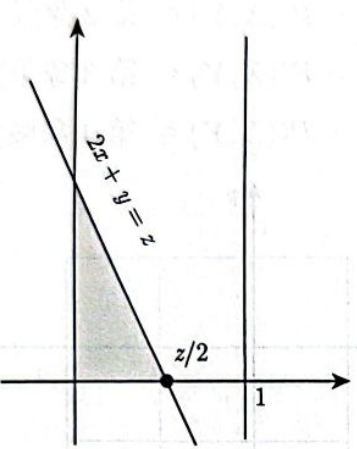
\includegraphics[scale = 0.2]{figures/figure3-53}
		\end{figure}
	\end{frame}
	
	\begin{frame}
		$0 \leqslant z<2, \quad F_{Z}(z)=\int_{0}^{z / 2} \mathrm{~d} x \int_{0}^{z-2 x} e^{-y} \mathrm{~d} y=\frac{z}{2}+\frac{1}{2} e^{-z}-\frac{1}{2},$
		
		\begin{figure}
			\centering
			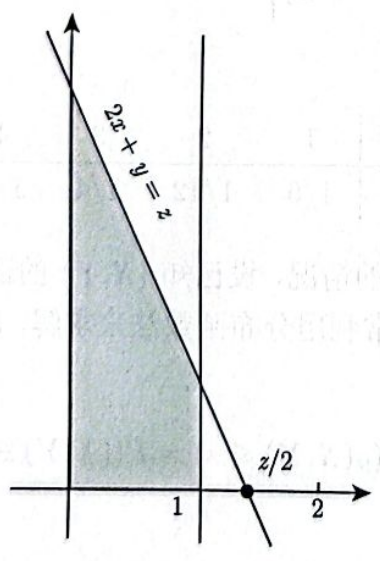
\includegraphics[scale = 0.2]{figures/figure3-54}
		\end{figure}
		$$
		z \geqslant 2, \quad F_{Z}(z)=\int_{0}^{1} \mathrm{~d} x \int_{0}^{z-2 x} e^{-y} \mathrm{~d} y=1-\frac{1}{2}\left(e^{2}-1\right) e^{-z}
		$$
		
		$$
		\therefore p_{Z}(z)=F_{Z}^{\prime}(z)=\left\{\begin{array}{ll}
			\frac{1}{2}-\frac{1}{2} e^{-z}, & 0 \leqslant z<2 \\
			\frac{1}{2}\left(e^{2}-1\right) e^{-z}, & z \geqslant 2 \\
			0, & z<0
		\end{array}\right. \text {. }
		$$
	\end{frame}
	
	\begin{frame}
		例 3.19 在区间$[0, 1]$随机投两点。求两点间距离$Z$的分布函数与密度函数。
		\begin{figure}
			\centering
			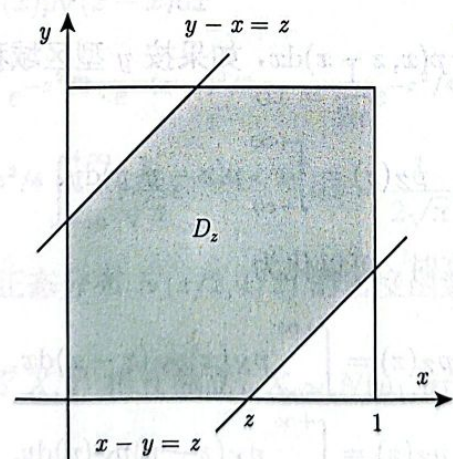
\includegraphics[scale = 0.37]{figures/figure3-55.jpg}
		\end{figure}
	\end{frame}
	
	\begin{frame}
		解 设两点坐标 $(X, Y)$, 则 $Z=|X-Y|,(X, Y)$ 服从 $[0,1] \times[0,1]$ 上的二维均匀分布, 其密度为
		
		$$
		p(x, y)=\left\{\begin{array}{cc}
			1, & 0 \leqslant x, y \leqslant 1 \\
			0, & \text { 其他 }
		\end{array}\right. \text { 。 }
		$$
		
		先求 $Z$ 的分布函数 $F_{Z}(z)$,
		
		$$
		F_{Z}(z)=P(Z \leqslant z)=P(|X-Y| \leqslant z)=\iint_{|x-y| \leqslant z} p(x, y) \mathrm{d} x \mathrm{~d} y,
		$$
		
		显然, $z<0$ 时, $F_{Z}(z)=0 ; z>1$ 时, $F_{Z}(z)=1 ; 0 \leqslant z \leqslant 1$ 时,
		
		$$
		\begin{aligned}
			F_{Z}(z) & =\iint_{|x-y| \leqslant z} p(x, y) \mathrm{d} x \mathrm{~d} y \\
			& =\iint_{|x-y| \leqslant z} \mathrm{~d} x \mathrm{~d} y=S_{D_{z}}=1-(1-z)^{2} \\
			& =2 z-z^{2},
		\end{aligned}
		$$
	\end{frame}
	
	\begin{frame}
		得到 $F_{Z}(z)=\left\{\begin{array}{cc}0, & z<0 \\ 2 z-z^{2}, & 0 \leqslant z \leqslant 1 \\ 1, & z>1\end{array}\right.$ 。
		
		$Z$ 的密度函数为
		
		$$
		p_{Z}(z)=F_{Z}^{\prime}(z)=\left\{\begin{array}{cc}
			2-2 z, & 0 \leqslant z \leqslant 1 \\
			0, & \text { 其他 }
		\end{array} 。\right.
		$$
	\end{frame}
	
	\begin{frame}
		1. 和与差的分布
		
		设 $(X, Y)$ 为二维随机变量, 其联合密度函数为 $p(x, y)$, 求 $Z=X+Y$ 的密度函数
		
		 $$p_{Z}(z)=\int_{-\infty}^{+\infty} p(x, z-x) \mathrm{d} x,$$
		 
		 如果按 $y$ 型区域积分, 可得
		
		$$
		p_{Z}(z)=\int_{-\infty}^{+\infty} p(z-y, y) \mathrm{d} y
		$$
		
		特别地, 若 $X, Y$ 相互独立时, 可以化为
		
		$$
		\begin{aligned}
			& p_{Z}(z)=\int_{-\infty}^{+\infty} p_{X}(x) p_{Y}(z-x) \mathrm{d} x \\
			& p_{Z}(z)=\int_{-\infty}^{+\infty} p_{X}(z-y) p_{Y}(y) \mathrm{d} y
		\end{aligned}
		$$
		
		以上两式称为卷积公式。 
	\end{frame}
	
	\begin{frame}
		类似可以得到差的分布公式, 设 $Z=X-Y$ 的密度函数 $p_{Z}(z)$, 则
		
		$$
		p_{Z}(z)=\int_{-\infty}^{+\infty} p(x, x-z) \mathrm{d} x=\int_{-\infty}^{+\infty} p(z+y, y) \mathrm{d} y 。
		$$
	\end{frame}
	
	\begin{frame}
		例 3.20 设随机变量 $X, Y$ 相互独立且有相同分布, 其密度函数均为
		
		$$
		p(x)=\left\{\begin{array}{cc}
			e^{1-x}, & x>1 \\
			0, & \text { 其他 }
		\end{array},\right.
		$$
		
		用卷积公式求 $Z=X+Y$ 的密度函数。 
	\end{frame}
	
	\begin{frame}
		解:由卷积公式, $Z=X+Y$ 的密度函数
		
		$$
		p_{Z}(z)=\int_{-\infty}^{+\infty} p_{X}(x) p_{Y}(z-x) \mathrm{d} x 。
		$$
		
		显然, $z$ 的可能取值范围是 $z>2$, 所以 $z \leqslant 2$ 时, $p_{Z}(z)=0$ 。
		
		由 $X$ 与 $Y$ 的密度函数可知, 仅当 $x>1$ 且 $z-x>1$ 即 $1<x<z-1$ 时, 上述积分的 被积函数不等于 0 , 于是
		
		$$
		p_{Z}(z)=\left\{\begin{array}{cc}
			\int_{1}^{z-1} e^{1-x} e^{1-(z-x)} \mathrm{d} x, & z>2 \\
			0, & \text { 其他 }
		\end{array}=\left\{\begin{array}{cl}
			(z-2) e^{2-z}, & z>2 \\
			0, & \text { 其他 }
		\end{array}\right. \text { 。 }\right.
		$$
	\end{frame}
	
	\begin{frame}
		例 3.21 设随机变量 $X, Y$ 相互独立且均服从标准正态分布, 求 $Z=X+Y$ 的密度 函数。
	\end{frame}
	
	\begin{frame}
		解 $X, Y$ 的密度函数均为
		
		$$
		p(t)=\frac{1}{\sqrt{2 \pi}} e^{-t^{2} / 2}, \quad-\infty<t<+\infty \text { 。 }
		$$
		
		由卷积公式
		
		$$
		\begin{aligned}
			p_{Z}(z) & =\int_{-\infty}^{+\infty} p_{X}(x) p_{Y}(z-x) \mathrm{d} x \\
			& =\frac{1}{2 \pi} \int_{-\infty}^{+\infty} e^{-x^{2} / 2} \cdot e^{-(z-x)^{2} / 2} \mathrm{~d} x=\frac{1}{2 \pi} e^{-z^{2} / 4} \int_{-\infty}^{+\infty} e^{-(x-z / 2)^{2}} \mathrm{~d} x \\
			& =\frac{1}{2 \sqrt{\pi}} e^{-z^{2} / 4} \int_{-\infty}^{+\infty} \frac{1}{\sqrt{\pi}} e^{-(x-z / 2)^{2}} \mathrm{~d} x=\frac{1}{2 \sqrt{\pi}} e^{-z^{2} / 4},
		\end{aligned}
		$$
		
		最后一个积分的被积函数是正态分布 $N(z / 2,1 / 2)$ 的密度函数, 所以积分值为 1 。由结果可 见, $Z \sim N(0,2)$ 。
	\end{frame}
	
	\begin{frame}
		一般情形, 可以推出, 若 $X, Y$ 相互独立, $X \sim N\left(\mu_{1}, \sigma_{1}^{2}\right), Y \sim N\left(\mu_{2}, \sigma_{2}^{2}\right)$, 则 $X+Y \sim$ $N\left(\mu_{1}+\mu_{2}, \sigma_{1}^{2}+\sigma_{2}^{2}\right)$ 。
		
		更一般的情形可以推广到 $n$ 维, 设 $X_{1}, X_{2}, \cdots, X_{n}$ 相互独立, $X_{i} \sim N\left(\mu_{i}, \sigma_{i}^{2}\right), i=$ $1,2, \cdots, n$, 则 $X_{1}+X_{2}+\cdots+X_{n} \sim N\left(\mu_{1}+\mu_{2}+\cdots+\mu_{n}, \sigma_{1}^{2}+\sigma_{2}^{2}+\cdots+\sigma_{n}^{2}\right)$ 。
	\end{frame}
	
	\begin{frame}
		2. 积与商的分布
		
		设 $Z=X Y$ 的密度函数 $p_{Z}(z)$, 则
		
		$$
		p_{Z}(z)=\int_{-\infty}^{+\infty} p\left(\frac{z}{y}, y\right) \frac{1}{|y|} \mathrm{d} y 。
		$$
		
		设 $Z=X / Y$ 的密度函数 $p_{Z}(z)$, 则
		
		$$
		p_{Z}(z)=\int_{-\infty}^{+\infty} p(z y, y)|y| \mathrm{d} y 。
		$$
	\end{frame}
	
	\begin{frame}
		3. $\max$ 与 $\min$ 的分布
		
		设随机变量 $X, Y$ 相互独立, 其分布函数分别为 $F_{X}(x)$ 和 $F_{Y}(y)$, 令 $M=\max (X, Y), N=$ $\min (X, Y)$, 以下我们推导 $M$ 和 $N$ 的分布函数。
		
		$M=\max (X, Y)$, 对于任意 $z, M \leqslant z$ 等价于 $X \leqslant z$ 且 $Y \leqslant z$, 因此
		
		$$
		\begin{aligned}
			F_{M}(z) & =P(M \leqslant z)=P(\max (X, Y) \leqslant z)=P(X \leqslant z, Y \leqslant z) \\
			& =P(X \leqslant z) P(Y \leqslant z)=F_{X}(z) F_{Y}(z) 。
		\end{aligned}
		$$
		
		类似有 $N=\min (X, Y)$, 对任意 $z, N>z$ 等价于 $X>z$ 且 $Y>z$,
		
		$$
		\begin{aligned}
			F_{N}(z) & =P(N \leqslant z)=P(\min (X, Y) \leqslant z)=1-P(\min (X, Y)>z) \\
			& =1-P(X>z, Y>z)=1-P(X>z) P(Y>z) \\
			& =1-\left[1-F_{X}(z)\right]\left[1-F_{Y}(z)\right] 。
		\end{aligned}
		$$
	\end{frame}
	
	\begin{frame}
		以上结果可以推广到 $n$ 个相互独立随机变量 $X_{1}, X_{2}, \cdots, X_{n}$ 的情形, 设 $X_{i}$ 的分布函 数为 $F_{X_{i}}\left(x_{i}\right), i=1,2, \cdots, n$, 令 $M=\max \left(X_{1}, X_{2}, \cdots, X_{n}\right), N=\min \left(X_{1}, X_{2}, \cdots, X_{n}\right)$, 则 $M$ 的分布函数 $F_{M}(z), N$ 的分布函数 $F_{N}(z)$ 分别为
		
		$$
		\begin{gathered}
			F_{M}(z)=F_{X_{1}}(z) F_{X_{2}}(z) \cdots F_{X_{n}}(z), \\
			F_{N}(z)=1-\left[1-F_{X_{1}}(z)\right]\left[1-F_{X_{2}}(z)\right] \cdots\left[1-F_{X_{n}}(z)\right] 。
		\end{gathered}
		$$
		
		特别地, 当随机变量 $\mathrm{X}_{1}, X_{2}, \cdots, X_{n}$ 相互独立且具有相同的分布函数 $F(x)$ 时, 有
		
		$$
		\begin{gathered}
			F_{M}(z)=[F(z)]^{n} \\
			F_{N}(z)=1-[1-F(z)]^{n} 。
		\end{gathered}
		$$
	\end{frame}
	
	\begin{frame}
		例 3.22 二维随机变量 $(X, Y)$ 在区域 $D=\{(x, y): 0<x, y<a\}$ 上服从均匀分布, 求 $M=\max (X, Y)$ 的概率密度函数。
	\end{frame}
	
	\begin{frame}
		解 $(X, Y)$ 的联合密度函数为
		
		$$
		p(x, y)=\left\{\begin{array}{cc}
			1 / a^{2}, & 0<x, y<a \\
			0, & \text { 其他 }
		\end{array}\right.
		$$
		
		可以求得
		
		$$
		\begin{aligned}
			& p_{X}(x)=\int_{-\infty}^{+\infty} p(x, y) \mathrm{d} y=\left\{\begin{array}{cc}
				1 / a, & 0<x<a \\
				0, & \text { 其他 }
			\end{array},\right. \\
			& p_{Y}(y)=\int_{-\infty}^{+\infty} p(x, y) \mathrm{d} x=\left\{\begin{array}{cc}
				1 / a, & 0<x<a \\
				0, & \text { 其他 }
			\end{array}\right.
		\end{aligned}
		$$
		
		可见, $p(x, y)=p_{X}(x) p_{Y}(y)$, 所以 $X, Y$ 相互独立, 均服从 $(0, a)$ 上的均匀分布, 由式 (3.26), $M=\max (X, Y)$ 的分布函数
		
		$$
		F_{M}(z)=F_{X}(z) F_{Y}(z)=\left\{\begin{array}{cc}
			z^{2} / a^{2}, & 0<z<a \\
			0, & \text { 其他 }
		\end{array},\right.
		$$
		
		
	\end{frame}
	
	\begin{frame}
		从而得到 $M=\max (X, Y)$ 的密度函数为
		
		$$
		p_{M}(z)=F_{M}^{\prime}(z)=\left\{\begin{array}{cc}
			2 z / a^{2}, & 0<z<a \\
			0, & \text { 其他 }
		\end{array}\right. \text { 。 }
		$$
		
		以上讨论随机变量 $X, Y$ 函数的分布时, $X, Y$ 同为离散型或同为连续型。若出现 $X, Y$ 一个是连续型, 另一个是离散型的情形, 可以用分布函数法, 把离散型随机变量的所有取值 看成样本空间的划分, 由全概率公式求解。
	\end{frame}
	
	\begin{frame}
		例 3.23 设随机变量 $X, Y$ 独立, 其中, $P(X=k)=1 / 3, k=1,2,3, Y$ 服从指数分布 $E(1)$, 求随机变量 $Z=X+Y$ 的概率密度函数。
	\end{frame}
	
	\begin{frame}
		解 $Y$ 的密度函数 $p_{Y}(y)=\left\{\begin{array}{cc}e^{-y}, & y \geqslant 0 \\ 0, & \text { 其他 }\end{array}\right.$, 设 $Z=X+Y$ 的分布函数为 $F_{Z}(z)$, 则
		
		\begin{align*}
			F_{Z}(z) & =P(Z \leqslant z)=P(X+Y \leqslant z) \\
			& =\sum_{k=1}^{3} P(X=k) P(X+Y \leqslant z \mid X=k) \\
			& =\frac{1}{3} \sum_{k=1}^{3} P(Y \leqslant z-k)=\frac{1}{3} \sum_{k=1}^{3} F_{Y}(z-k), \\
		\end{align*}
	\end{frame}
	\begin{frame}
		\begin{align*}
			p_{Z}(z) & = F_{Z}^{\prime}(z) \\
			& =\frac{1}{3}\left[p_{Y}(z-1)+p_{Y}(z-2)+p_{Y}(z-3)\right] \\
			& = \begin{cases}
				0, & z<1 \\
				e^{1-z} / 3, & 1 \leqslant z<2 \\
				\left(e^{1-z}+e^{2-z}\right) / 3, & 2 \leqslant z<3 \\
				\left(e^{1-z}+e^{2-z}+e^{3-z}\right) / 3, & z \geqslant 3
			\end{cases}
		\end{align*}
	\end{frame}
\end{document}